\documentclass[../manuale-utente.tex]{subfiles}

\begin{document}

\subsection{Requisiti}%
\label{sub:requisiti}

\begin{description}
    \item[Browser:] Google Chrome 50, Firefox 48, Safari 9.1.
    \item[Necessario:] JavaScript.
\end{description}


\subsection{Manuale d'uso}%
\label{sub:manuale-uso-web}

\subsubsection{Pagina home}%
\label{subs:pagina-home}

\begin{figure}[H]
    \centering
    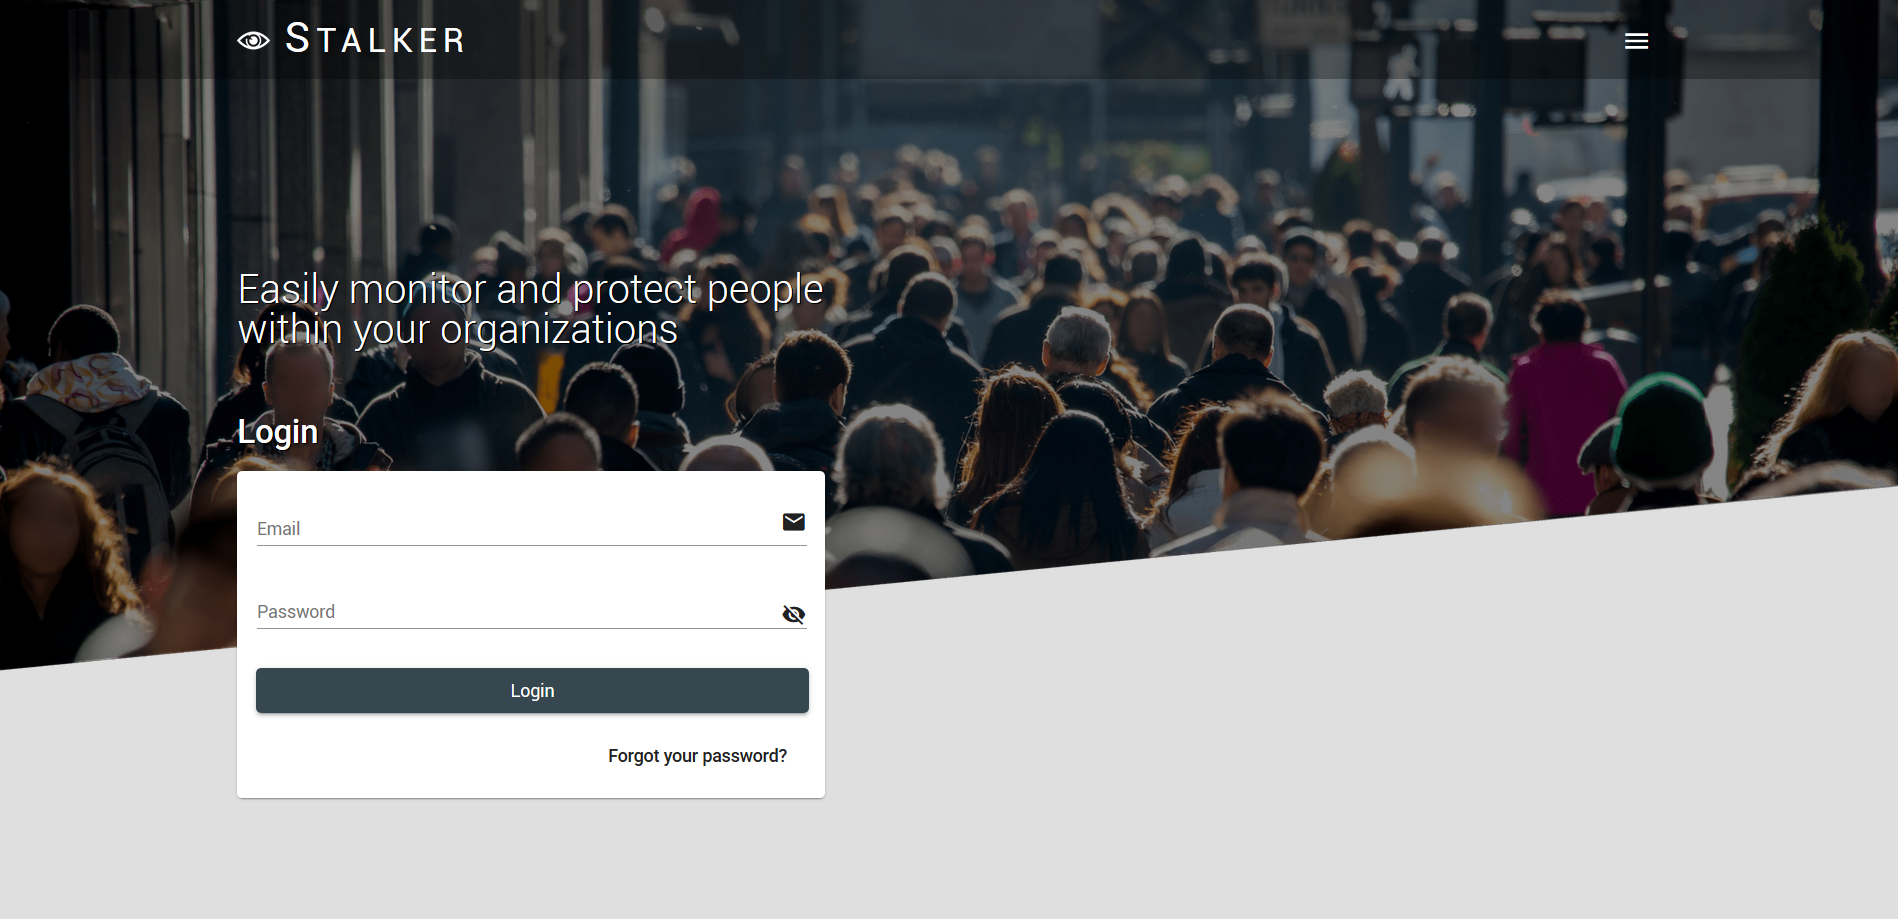
\includegraphics{img/web-app/pagina-home.PNG}
    \caption{Pagina di accesso}%
    \label{fig:web-app-pagina-accesso}
\end{figure}

\textbf{Endpoint}: localhost:4200/home
Lorem ipsum

\paragraph{Accesso alla web application}%
\label{par:accesso-alla-web-application}

\begin{figure}[H]
    \centering
    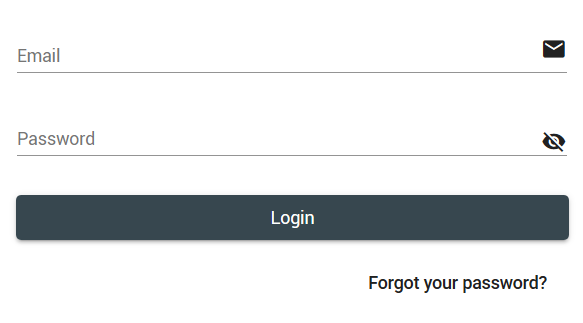
\includegraphics{img/web-app/accesso-web-app.png}
    \caption{Pagina di registrazione}%
    \label{fig:web-app-accesso}
\end{figure}

Lorem ipsum

\paragraph{Recupero password}%
\label{par:recupero-password}

\begin{figure}[H]
    \centering
    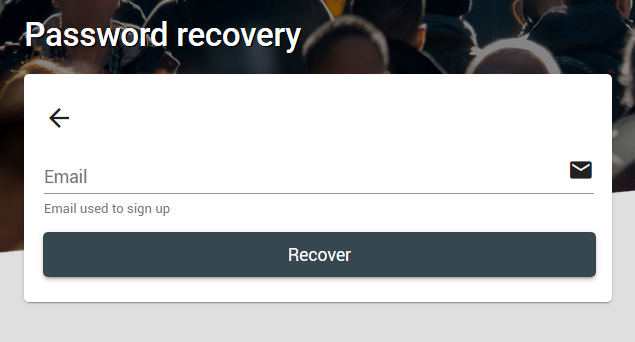
\includegraphics{img/web-app/recupero-password.PNG}
    \caption{Recupero password}%
    \label{fig:web-app-recupero-password}
\end{figure}

Lorem ipsum

\subsubsection{Visualizza profilo personale}%
\label{subs:visualizza-profilo-personale}

\begin{figure}[H]
    \centering
    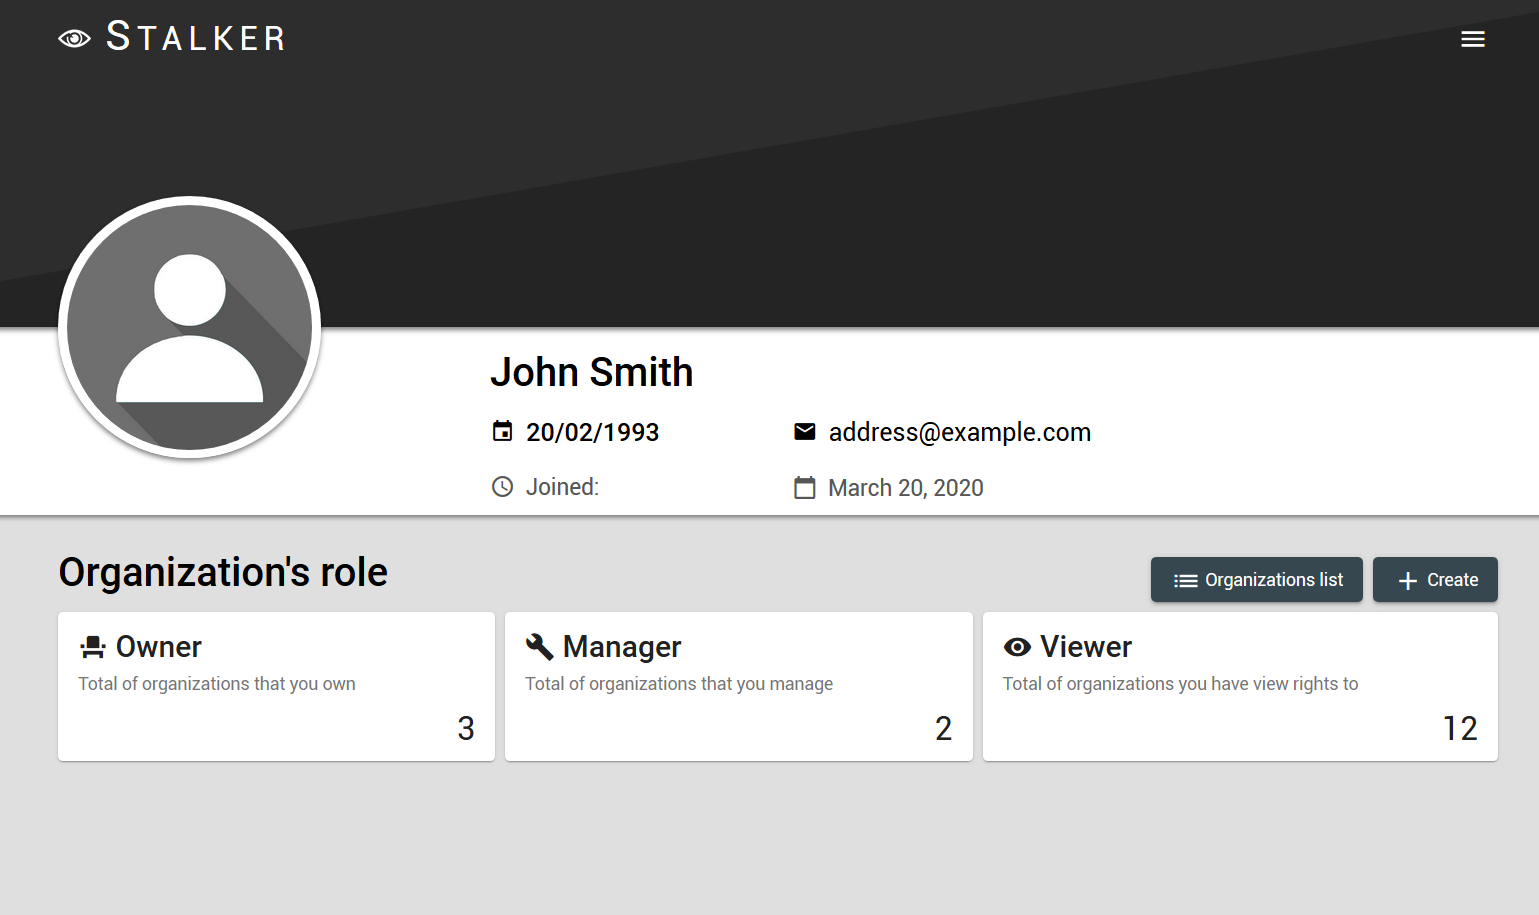
\includegraphics{img/web-app/visualizza-profilo-personale.PNG}
    \caption{Visualizza profilo personale}%
    \label{fig:web-app-visualizza-profilo-personale}
\end{figure}

\textbf{Endpoint}: localhost:4200/users/:id
Lorem ipsum

\subsubsection{Visualizza organizzazioni}%
\label{subs:visualizza-organizzazioni}

% \begin{figure}[H]
%     \centering
%     \includegraphics{img/web-app/visualizza-organizzazioni.png}
%     \caption{Visualizza organizzazioni}%
%     \label{fig:web-app-visualizza-organizzazioni}
% \end{figure}

\textbf{Endpoint}: localhost:4200/organizations
Lorem ipsum

\paragraph{Visualizza dettagli organizzazione}%
\label{par:visualizza-dettagli-organizzazione}

\begin{figure}[H]
    \centering
    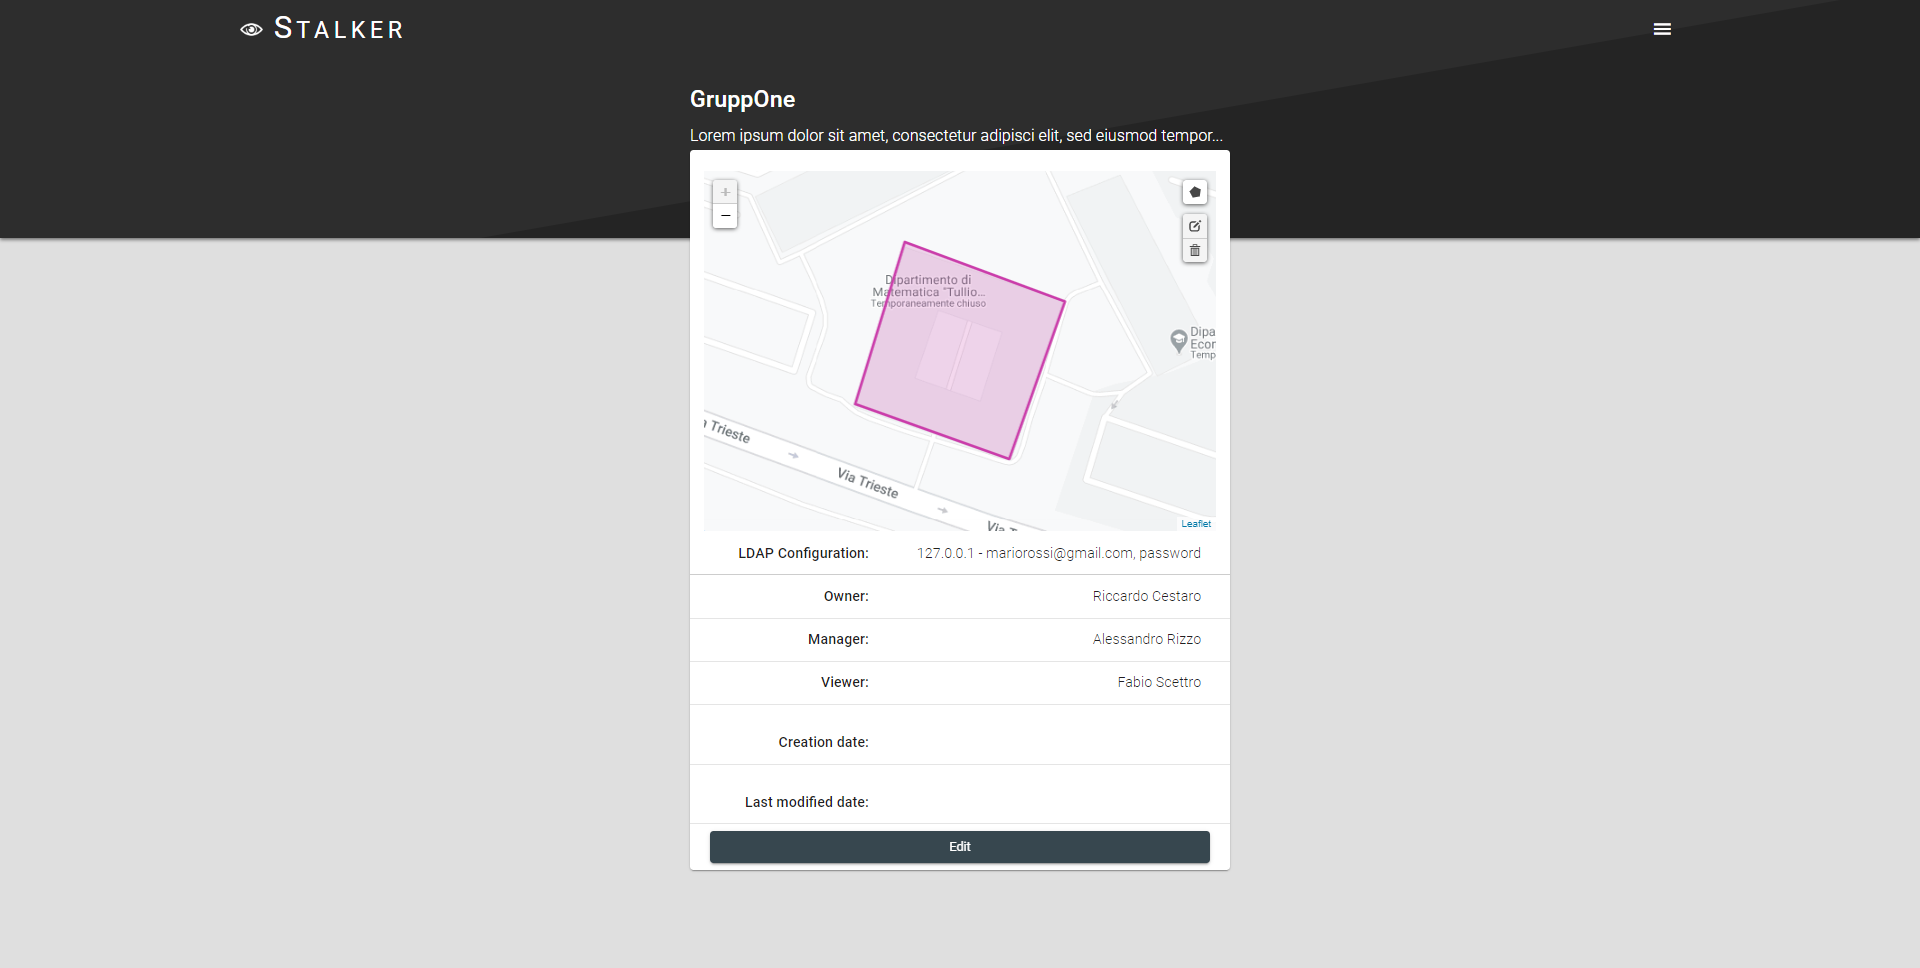
\includegraphics{img/web-app/visualizza-dettagli-organizzazione.png}
    \caption{Visualizza dettagli organizzazione}%
    \label{fig:web-app-visualizza-dettagli-organizzazione}
\end{figure}

\textbf{Endpoint}: localhost:4200/organizations/:id
Lorem ipsum

% Visualizza: (aggiungere un'immagine per ogni funzionalità) --> edit-organization
% - luoghi da una mappa interattiva
% - LDAP configuration
% - managers, owners e viewers
% - ecc..


\subsubsection{Modifica dettagli organizzazione}%
\label{subs:modififica-dettagli-organizzazione}

% \begin{figure}[H]
%     \centering
%     \includegraphics{img/web-app/modifica-dettagli-organizzazione.png}
%     \caption{Modifica dettagli organizzazione}%
%     \label{fig:web-app-modifica-dettagli-organizzazione}
% \end{figure}

\textbf{Endpoint}: localhost:4200/organizations/:id/edit
Lorem ipsum

% add other functionalities 

\end{document}
